\begin{frame}
  \frametitle{Concurrent Object Deallocation}

  \begin{enumerate}
  \item mark root reference as zombie
  \item recursively revoke all children in inheritance tree:
  \item[$\Rightarrow$] informs reference holders, ack.\ as continuation
  \item broadcast task to all active cores
  \item[$\Rightarrow$] safeguard against temporary references
  \item call async.\ deletion method of the object
  \item[$\Rightarrow$] delayed by monitor until all pending tasks done,\\
    return memory to parent, ack.\ as continuation
  \item respond via ack.\ continuation
  \end{enumerate}
\end{frame}

\begin{frame}[fragile]
  \frametitle{Object Invocation: User Side Proxy Pointer}

    \begin{semiverbatim}
void Adder::add(Portal* p, Future f, int , int b) \{
  p->invoke(this->obj, ADDERPROT, ADD, f, a, b); 
\}

// \ldots in app's idle loop:
Portal* res = wait();
if (res) res->handleResponse(); // pushes results to f
    \end{semiverbatim}  

  \begin{itemize}
  \item \texttt{p} same role as tasklets, larger message
  \item \texttt{Future f} depends on user's programming model
  \item based on C++11 variadic templates and \texttt{operator<<}
  \end{itemize}
\end{frame}

\begin{frame}
  \frametitle{Many Threads Operating System}
  %\framesubtitle{}

  \begin{center}
    
\includegraphics[scale=0.3]{mythos-logo}
  \end{center}
  \vspace{0.5cm}

  \begin{itemize}
  \item[\textbf{Ziel}] \alert{dynamische} HPC Anwendungen auf \alert{Vielkern-Prozessoren}
  \item[\textbf{Fokus}] schnelle Thread-Verwaltung
  \item durchschnittlicher Durchsatz statt worst-case Latenz
  \item BMBF Projekt\footnote{Fördernummer BMBF 01IH13003} von Uni Ulm, mit Uni Siegen, BTU Cottbus, \\ Alcatel-Lucent Deutschland AG, HLRS Stuttgart
  \end{itemize}
\end{frame}

\begin{frame}
  \frametitle{Multi- versus Many-Core}

  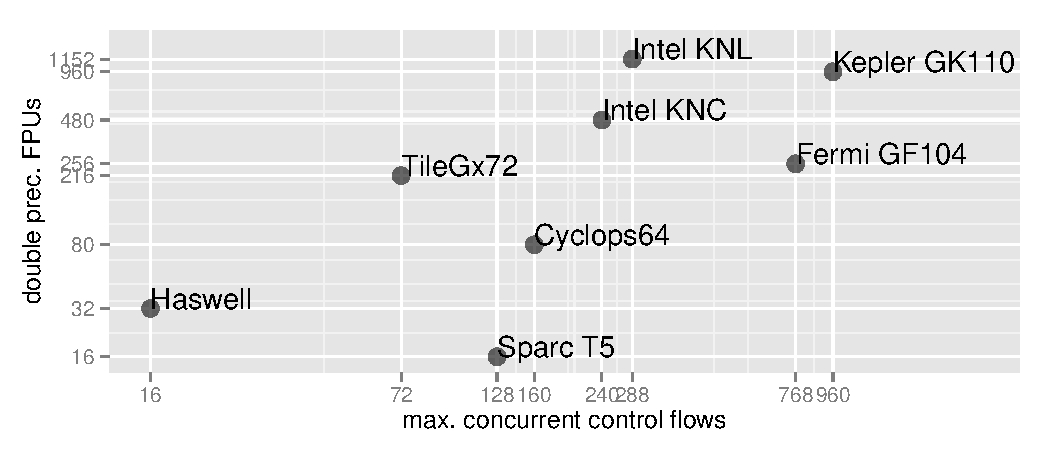
\includegraphics[height=5cm]{figures/manycore}

  \begin{itemize}
  \item max. paralleler Durchsatz in geg. Power- \& Platz-Budget 
  \item Energie- \& Platzeffizienz statt Single-Thread Performance 
  \item[$\Rightarrow$] \alert{Durchsatz nur durch Aufgaben- und Daten-Parallelität }
  \end{itemize}
\end{frame}

\begin{frame}
  \frametitle{Zielarchitektur: Intel XeonPhi KNC}
  %\framesubtitle{Intel Xeon Phi Knights Corner}

  \begin{center}
    %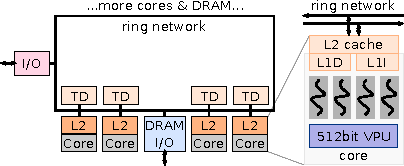
\includegraphics[height=2cm]{figures/hw-xeonphi}
    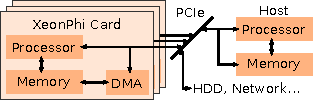
\includegraphics[height=2cm]{figures/hw-xeonphi-host}
  \end{center}

  \begin{itemize}
  \item 60 Kerne: In-Order, keine Sprungvorhersage, 2 Takte Instruction Decode
    % consequence: low single-thread performance, sensitive to branches
  \item 4 HW Threads per Core: gemeinsamer L1+L2 Cache,\\ 
    gemeinsamer TLB, keine Global Pages, keine TLB PCIDs 
    % consequence: switching between address spaces is expensive
  \item 8GiB Hauptspeicher: $<$35 MiB per Thread,\\
    Cohency Latenz $>$200 Takte, pseudo-uniform, kein MWAIT
    % consequence: cannot be used like pure distributed memory system, synchronisation and communication via shared memory curbed by slow CC  
  \item PCIe Karten: unterstützen custom OS Kernel,\\
    Kommunikation mit Host über gem. Speicher
    % consequence: easy to experiment with
  \item[$\Rightarrow$] \alert{Ideale Worst-Case Plattform!?}
  \end{itemize}
\end{frame}

\begin{frame}
  \frametitle{Szenario I: HPC Simulationen}
  \framesubtitle{Moleküldynamik (HLRS), Strömungen und Elektrodynamik (Uni Siegen)}

  \begin{itemize}
  \item eine Anwendung besitzt ``alle'' Kerne und Speicher
  \item Aufgabenverwaltung und Kommunikation auf Anwendungsebene
  \item dynamische Speicherverwaltung
  \end{itemize}

  \begin{block}{Anforderungen}
    \begin{itemize}
    \item effizientes Warten statt Polling (min Energie, min Contention)\\
      Semaphore/Futex \texttt{wait}, \texttt{signal}
    \item viele Threads manipulieren gemeinsamen Adressraum (IO,PGAS,DSM)\\
      \texttt{mmap}, \texttt{mremap}, \texttt{mprotect}
    \end{itemize}
  \end{block}
\end{frame}

\begin{frame}
  \frametitle{Szenario II: Compute Cloud}
  \framesubtitle{Verteilte Medienverarbeitung (Alcatel/CenoLabs)}

  \begin{itemize}
  \item dynamisch konfigurierter Datenfluss-Graph
  \item Knoten aktiviert durch Input Daten, laufen in Isolation+Zeitschranke
  \item Cloud Manager bewegt Daten, migriert Knoten für min. Energie
  \end{itemize}

  \begin{block}{Anforderungen}
    \begin{itemize}
    \item viele Threads mit eigenem Adressraum erzeugen und aktivieren\\
      \texttt{create}, \texttt{destroy}, \texttt{activate} mit Zeitschranke
    \item Manager manipuliert fremde Adressräume, z.B. zero-copy comm\\
      \texttt{mmap}, \texttt{mremap}, \texttt{mprotect} auf Kind-Threads
    \item Weiterleiten der Systemaufrufe, Exceptions etc. an Manager\\
      \texttt{event queue}
    \end{itemize}
  \end{block}
\end{frame}

